% \IUref{IUAdmPS}{Administrar Planta de Selección}
% \IUref{IUModPS}{Modificar Planta de Selección}
% \IUref{IUEliPS}{Eliminar Planta de Selección}


% Copie este bloque por cada caso de uso:
%-------------------------------------- COMIENZA descripción del caso de uso.

%\begin{UseCase}[images/CU21]{UCX}{Nombre del Caso de uso}{
	\begin{UseCase}{CU21}{Alta de un curso}{
		Resumen:Cuando el Gerente de Sucursal va a registrar un curso en el sistema, se registran los datos: nombre de curso, costo, horario, fecha de inicio,area, fecha de termino,nombre de instructor y su  horario en formato 24:00. Este Curso sera asociado a una area y a un instructor, la cual será determinada en su regístro por el Gerente de Sucursal. Una vez Validado los 8 campos (todos obligatorios), sera registrado el curso en el sistema.
		\begin{figure}
  		\centering
   		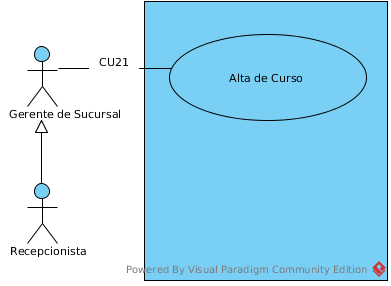
\includegraphics[width=0.4\textwidth]{images/CU21}
  		\caption{CU21 Alta de Curso}
		\end{figure}
	}
		\UCitem{Versión}{1.0}
		\UCitem{Actor}{Gerente de Sucursal}
		\UCitem{Propósito}{Alta de cursos por el Gerente de Sucursal.}
		\UCitem{Entradas}{nombre de curso, costo, horario, fecha de inicio,area, fecha de termino,nombre de instructor y su  horario en formato 24:00}
		\UCitem{Origen}{Teclado}
		\UCitem{Salidas}{nombre de curso, costo, horario, fecha de inicio,area, fecha de termino,nombre de instructor y su  horario en formato 24:00 }
		\UCitem{Destino}{Pantalla}
		\UCitem{Precondiciones}{El curso no debe de estar registrado en el sistema con los mismas descipciones, ademas no debe coincidir otro curso ya registrado con el horario, la fecha de inicio, la fecha de termino, el area, y el instructor ingresados previamente.}
		\UCitem{Postcondiciones}{El Gerente de Sucursal dara de alta un registro mas al sistema.}
		\UCitem{Errores}{Que no se tenga memoria disponible en el Disco.}
		\UCitem{Tipo}{Caso de uso primario}
		\UCitem{Observaciones}{Los cursos solo pueden ser registrados por un Gerente de Sucursal.}
		\UCitem{Autor}{Carrillo Mendoza Martín Alejandro.}
		\UCitem{Reviso}{Carrillo Mendoza Martín Alejandro.}	
	\end{UseCase}
	\newpage
	\begin{UCtrayectoria}{Principal}
	\UCpaso[\UCactor] Ingresa a la pagina web de \IUref{IU21.0}{Pantalla de Control de Acceso}\label{CU21.0Login} y proporciona su correspondiente nombre de usuario (username) y contraseña (password) para acceder al sistema.
		\UCpaso Válida que el actor se encuentre dado de alta en el sistema. Se utiliza la regla \BRref{BR117}{Determinar si el usuario tiene acceso al sistema.} \Trayref{A}.
		\UCpaso Despliega la \IUref{IU21.1}{Pantalla de Alta de un curso en el sistema} que es la pestaña principal del acceso como gerente de sucursal, en ella se encuentran los campos: nombre de curso, costo, horario, fecha de inicio,area, fecha de termino,nombre de instructor y su  horario en formato 24:00, todos ellos obligatorios para el registro de un curso en el sistema.
	\UCpaso[\UCactor] Al solicitar el registro de un curso a la base de datos,selecciona la pestaña " Alta de Curso  " de la IU21.1 de Menú principal.
	\UCpaso El sistema carga una nueva pagina con los campos: nombre de curso, costo, horario, fecha de inicio,area, fecha de termino,nombre de instructor y su  horario en formato 24:00.
	\UCpaso[\UCactor] Introduce los datos del curso a dar de alta, con su respetivo formato y tipo de dato solicitado, estos son: nombre de curso(varchar), costo(float), fecha de inicio(DATE), fecha de termino(DATE), costo(float).
    \UCpaso[\UCactor] Selecciona el nombre del instructor a impartir nuevo curso.
	\UCpaso[\UCactor] Selecciona los dias ala semana en los que se imparte nuevo curso.
	\UCpaso[\UCactor] Selecciona la hora en que se impartira un curso (los dias ya seleccionados previamente).
	\UCpaso[\UCactor] Selecciona el area donde se impartira un curso.
	\UCpaso[\UCactor] Confirma el Alta de curso al sistema dando click al boton \IUbutton{Enviar} de \label{IU21.1 Alta Curso}.
	\UCpaso Verifica que todos los campos esten llenos ademas con el formato y tipo correspondiente a los datos ubucados en la base de datos. \BRref{BR118}{Validar los datos de un formulario} \Trayref{B}.
		
		\UCpaso Almacena los datos en la base de datos.
		\UCpaso Muestra el \IUref{UI21}{Registro Exitoso de nuevo curso.}\Trayref{C}.
		\UCpaso Regresa a la pantalla principal de acceso a gerente de sucursal\IUref{IU21.1}{Pantalla de acceso a Gerente de Sucursal}.
\end{UCtrayectoria}

\begin{UCtrayectoriaA}{A}{El actor no introduce nombre de usuario (username) y contraseña (password) para poder ingresar al sistema.}
			\UCpaso Muestra el mensaje {\bf MSG21.0-}``Usuario [{\em y/o}] contraseñas no validos.''.
			\UCpaso[\UCactor] Oprimé el botón \IUbutton{Aceptar}.
			\UCpaso Rgresa a la pantalla principal de acceso a gerente de sucursal\IUref{IU21.1}{Pantalla de acceso a Gerente de Sucursal}.
		\end{UCtrayectoriaA}

		\begin{UCtrayectoriaA}{B}{Almenos un campo no esta lleno o no tiene formato adecuado}
			\UCpaso Muestra el mensaje {\bf MSG21.1-}``Uno o más [{\em campos}] no tienen el formato adecuado''.ademas que se tiene obligatoriamente que llenar todos los campos.
			\UCpaso[\UCactor] Oprime el botón \IUbutton{Aceptar}
			\UCpaso[] Termina el caso de uso.
		\end{UCtrayectoriaA}
		
		\begin{UCtrayectoriaA}{C}{El alta del curso no fue realizada }
			\UCpaso Muestra el Mensaje {\bf MSG21.2-}El Curso [{\em nombre de curso, costo, horario, fecha de inicio,area, fecha de termino,nombre de instructor y su  horario en formato 24:00 }] no registrado en el sistema, compruebe memoria en el Disco.
			\UCpaso[\UCactor] Oprime el botón \IUbutton{Aceptar}
			\UCpaso[] Termina el caso de uso.
		\end{UCtrayectoriaA}	
%-------------------------------------- TERMINA descripción del caso de uso.